\chapter{A method to correct upwelling longwave radiation to estimate hemispherical urban surface temperature}

\section{Introduction}
Thermal infrared (TIR) remote sensing of land surface temperature (T\textsubscript{surf}) has emerged as a primary research focus in climatology, as researchers seek to better describe spatiotemporal patterns of T\textsubscript{surf} globally and better understand how anthropogenic modification of earth's surface influences land T\textsubscript{surf} with links to the climate at-large. Over the last two decades, use of thermal remote sensing of surface climates has expanded significantly --- both in terms of the volume and breadth of remote sensed study and its explicative importance in climatology as a discipline. Thermal remote sensing of earth's surface has applications over a wide range of disciplines: from informing micro-, urban-, and global-scale climate models, to aiding decision making and mitigation praxis with respect to climate change and the \gls{uhi}. 

Within urban climatology, a combination of satellite, aerial, and ground-based thermal remote sensors have been integral in elucidating the spatial \cite{Roth1989}, temporal \cite{Peng2012}, and geometric \cite{Voogt1997} effects of the built environment on land T\textsubscript{surf}; in evaluating and partitioning urban surface energy balances \cite{BastiaanssenW.G.M.1998, Yamaguchi2005} and; in characterizations of the relationship between surface and \gls{blayer} air temperatures (T\textsubscript{air}) \cite{Stoll1992}. These advances have been aided by substantial improvements in sensor ground, spectral, and radiometric resolutions, and by the proliferation of both large-scale public satellite remote sensing campaigns and low-cost aerial and near-ground thermography. However, in spite of it's widespread usage, several questions concerning the use and validity of urban remote thermal remote sensing, first posed in Roth et al. 1989 \cite{Roth1989}, have yet to be sufficiently answered, viz,

\begin{enumerate}
	\item What is the nature of the surface 'seen' by a thermal remote sensor?
	\item How does T\textsubscript{surf} observed by a remote sensor relate to the 'true' temperature governing the surface-atmosphere interface?
\end{enumerate}

\noindent In this paper, we seek to examine question two by introducing and evaluating a method for atmospheric and emissivity correction of near-ground hemispherical TIR --- measured via \gls{pyrg} --- for hemispherical radiometric temperature (T\textsubscript{hem}) retrieval. These measures are common to most urban energy balance assessments and thus constitute a hitherto untapped method for urban T\textsubscript{surf} analysis. A companion paper responds to question one through an analysis of a climatology of T\textsubscript{hem} and derived surface UHI (sUHI), to quantify geometric and temporal biases across multiple methods for remote sensing of urban T\textsubscript{surf}.

\section{Atmospheric effects on TIR}

Although most thermal remote sensors operate within one of the \gls{atmwind}[s] --- where atmospheric effects are greatly reduced --- virtually any remote sensed TIR signal is subject to radiative effects from the layer of atmosphere between the surface and the sensor. Over much of the thermal infrared \gls{waveband} the atmosphere emits radiation and absorbs a fraction of radiation emitted by the surface. Thus, a remote sensed TIR signal almost certainly not equal to the ground emitted signal. For an isothermal, homogeneous surface-atmosphere system, at-sensor spectral radiance at height ($z$) can be described by a function deviating from a Planck curve at T\textsubscript{surf} based on the spectral transmittance of the intervening atmosphere, with the magnitude of that deviation governed by the difference between Planck curves at T\textsubscript{surf} and the ambient T\textsubscript{air}. As shown for two path geometries in \ref{spectairtsurf} for an atmosphere with water vapor content of  12 g/m\textsuperscript{3} and aerosol and trace gas profiles from the mid-latitude summer standard atmosphere, an at-sensor spectral radiance signal deviates significantly from the surface emitted spectral radiance curve. A less transmissive atmosphere increases the potential for deviation in the at-sensor signal from the ground emitted signal, while the difference between T\textsubscript{air} and T\textsubscript{surf} determines the resulting magnitude of atmospheric influence on the spectral TIR signal.

\begin{figure}[!ht]
	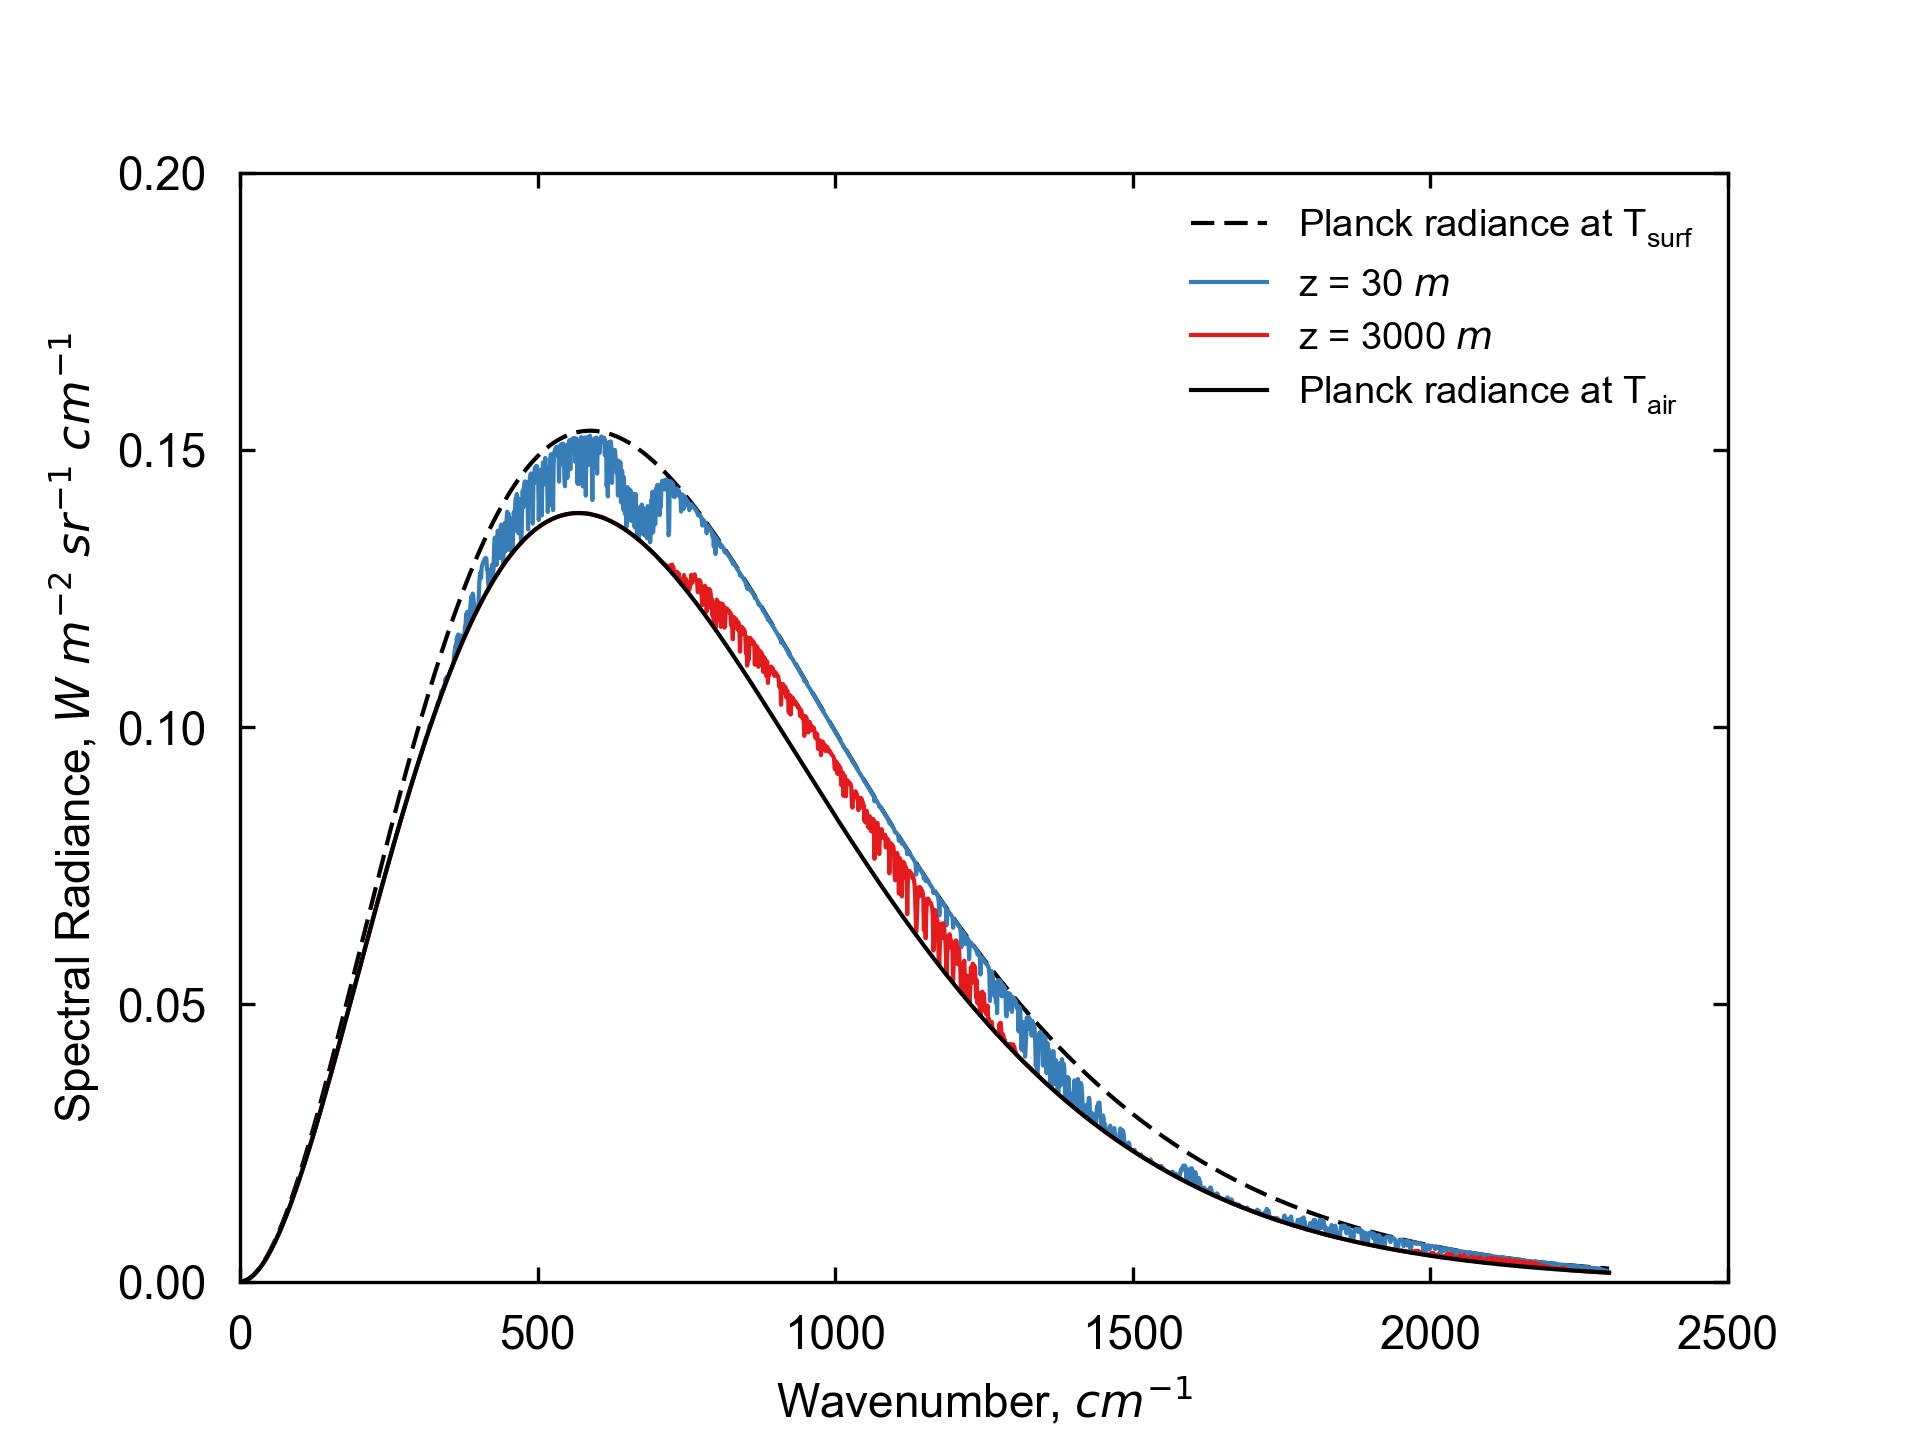
\includegraphics[width=\textwidth]{spectairtsurf}
	\caption{At-sensor spectral directional radiances computed in MODTRAN 4.1 \cite{Berk1987} for short (30m) and long (3000m) path lengths (z) with Planck curves indicating spectral radiances at T\textsubscript{air} = 305 K and T\textsubscript{surf} = 295 K.}
	\label{spectairtsurf}
\end{figure}

Atmospheric effects can lead to differences between the 'true' radiometric T\textsubscript{surf} and the remote sensed T\textsubscript{surf} of over 10 k for satellite platforms \cite{Cooper1989} and over 6 K for near-ground sensors \cite{Meier2011}. Moreover, because atmospheric and emissivity effects are a function of non-uniform and spatiotemporally variant surface and atmospheric properties, their associated errors change depending on instrument type, surface-sensor geometry, study location, and ambient conditions. As intersite and time-sequential analysis is a significant goal of most thermal remote sensed studies (urban or otherwise) these effects cannot be ignored.

Spectral transmission of longwave radiation through a given layer of atmosphere is dependent on total column absorber content (the principal broadband TIR absorbers are H\textsubscript{2}0, C0\textsubscript{2}, and to a lesser extent 0\textsubscript{3}, N\textsubscript{2}0, CO, CH\textsubscript{4}, and 0\textsubscript{2} \cite{Miskolczi1993}). Holding vertical absorber content constant, variation in band-by-band TIR transmittance with path length is greatest at urban scales (approximately 1 to 50 meters), where transparent spectral bands can quickly become opaque with small changes in path length or absorber content - illustrated in figure \ref{spectransheight}. Thus, transmittance of TIR near the surface is highly dependent on surface-sensor geometry, instrument spectral response, and atmospheric absorber content. Indeed, accurate assessment of atmospheric influence on TIR may be most complex when measured near the surface.

\begin{figure}[H]
	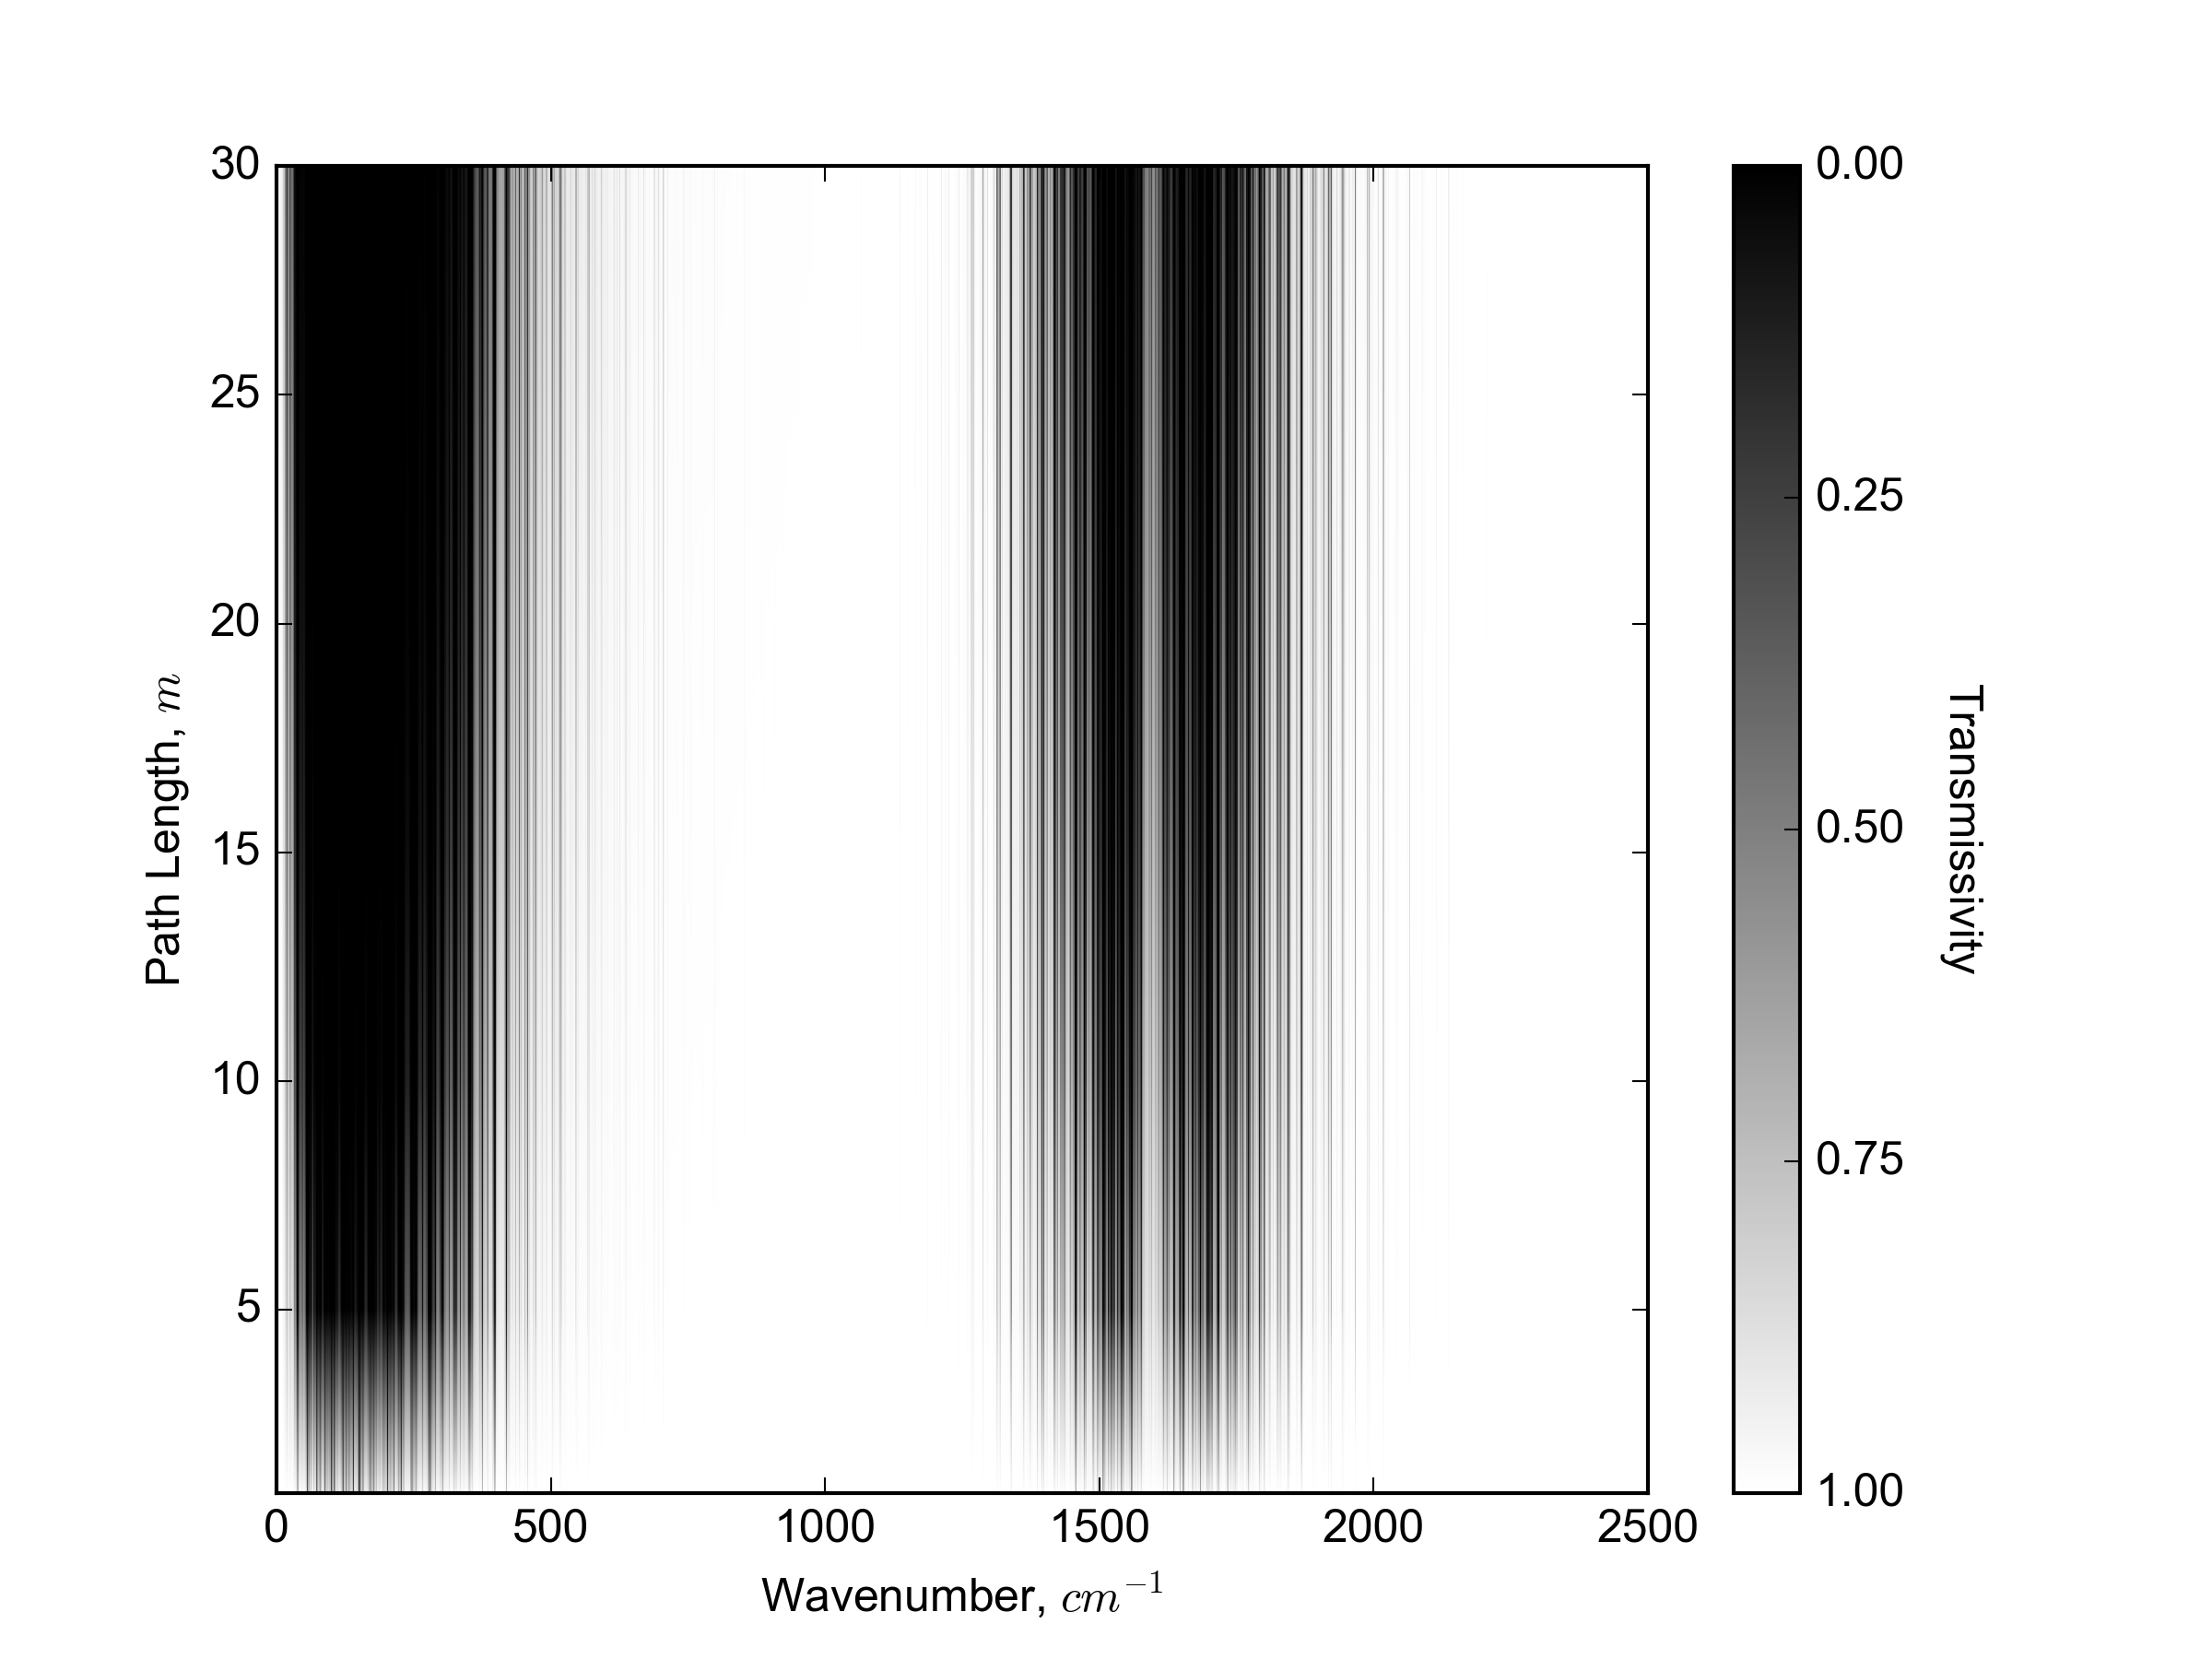
\includegraphics[width=\textwidth]{spectransheight}
	\caption{Spectral transmission of water vapor as a function of height. Black and grey shading indicate opaque (0\% transmittance) and transparent (100\% transmittance) bands respectively. Redo this figure with wavelength and colorbar no totle and the tick marks in back on the outside?}
	\label{spectransheight}
\end{figure}

Radiation passing through a layer of atmosphere from an emitting surface can be described in a number of ways. \textit{Spectral directional radiance} $ R (\lambda)$, at height $ z $ and from a direction defined by zenith angle \(\theta\), and azimuth angle \(\phi\) is commonly written as

\begin{equation}
R^\uparrow_z (\lambda, \theta, \phi) = \tau_\lambda \epsilon R^\uparrow_0(\lambda) + (1-\epsilon) R^\downarrow_{sky} (\lambda) + (1-\tau_\lambda) R^\uparrow_{atm}(\lambda)
\end{equation}

\noindent where \(\epsilon\) is surface emissivity, \(\tau\)\textsubscript{\( \lambda \)} is spectral "slab" transmittance through the layer between the emitting surface $( z  = 0) $ and $ z $. The same spectral TIR signal, as measured by a narrow-FOV sensor mounted at height $ z $, passes through an instrument shield (or dome) with spectral transmittance \(\tau_d\), and is integrated over the sensor waveband (bounded by \(\lambda_1\) and \(\lambda_2\)) to yield a \textit{directional radiance} $L'$ as 'seen' by the sensor

\begin{equation}
L'_z (\theta, \phi) = \int_{\lambda_1}^{\lambda_2} \tau_d(\lambda) R^\uparrow_z(\lambda) ~ d\lambda
\end{equation}

\noindent which, integrated over the hemisphere with respect to zenith \(\theta\) angle and azimuth \(\phi\) angle, yields an \textit{irradiance} $ L $ at height $ z $,

\begin{equation}
L_z = \int_{0}^{2\pi} \int_{0}^{\pi/2} L_z'(\theta, \phi) ~ \cos\theta \sin\theta ~ d\theta d\phi
\end{equation}

\subsection{Relating TIR and surface temperature}

TIR received by a remote sensor can be related to the emitting body's temperature in a number of ways --- each producing different conceptions of T\textsubscript{surf} from different instrument and sensor types. As such, the term "surface temperature" with respect to a remote sensed TIR is vague and can refer to several definitions of "surface" and "temperature" Thus, proper terminology must be attached to land T\textsubscript{surf} inferred from TIR. Definitions and nomenclature conventions for multiple methods for T\textsubscript{surf} retrieval are discussed at length in Norman \& Becker, (1995)\cite{Norman1995}.

Directional radiance $ L'_z $ detected from a narrow-FOV sensor operating over waveband (\(\lambda_1\) --- \(\lambda_2\)) and viewing the surface from some orientation described by \(\theta\), \(\phi\) can be used to infer a \textit{directional brightness temperature} T'\textsubscript{bright}(\(\theta\), \(\phi\)) via an inversion of the Planck function multiplied by normalized sensor response integrated over the sensor waveband,

\begin{equation}
L'_z(T'_{bright} (\theta, \phi)) = \bigints_{\lambda_1}^{\lambda_2} \cfrac{f(\lambda) C_1}{\pi \lambda^5 \left( \exp\left(\cfrac{C_2}{\lambda T'_{bright} (\theta, \phi)}\right)\right)}
\end{equation}

\noindent where C\textsubscript{1} = $ 3.7404 \cdot 10^8 $ $ W\mu^4 m^{-2} $, C\textsubscript{2} = $ 14387 \mu K $, and relative sensor response $ r(\lambda) $ normalized via,

\begin{equation}
1 ~ =  \int_{\lambda_1}^{\lambda_2} r(\lambda) ~ d\lambda
\end{equation}

Similarly irradiance $L_z$ received by a broadband hemispherical sensor (such as a pyrgeometer), can be used to infer a \textit{hemispherical brightness temperature} T\textsubscript{bright} through an inversion of the Stefan-Boltzmann law,

\begin{equation}
\label{stefb1}
L_z = \overline{r} (\sigma T_{bright}^4)
\end{equation}

\noindent where $ \sigma $ is the Stefan-Boltzmann constant and $ \overline{r} $ is Planck weighted average broadband sensor response computed as,

\begin{equation}
\overline{r} = \cfrac{\int R(\lambda) ~ r(\lambda)}{\int R(\lambda)}
\end{equation}

\noindent with $ R(\lambda) $ computed from a Planck function at an approximated $T_{bright}$. 

In addition, a simple approximation of $T_{bright}$ can be inferred from directional radiance using equation \ref{stefb1} by replacing $ L_z $ with $L'_z$ multiplied by a constant. This method is commonly used to infer T\textsubscript{bright} from infrared thermometers (IRT) operating over the atmospheric window (where atmospheric correction magnitudes are small and T\textsubscript{bright} is a reasonably accurate approximation of T\textsubscript{surf}). However, constants must be calibrated for the range of expected T\textsubscript{surf} as the relationship between $ L_z $ and $L'_z$  is not perfectly linear.

Inversions of uncorrected directional radiances or irradiances using the Planck function or the Stefan-Boltzmann law yield a temperature equal to that of a blackbody emitting the same amount of radiation as detected by the sensor. Since $ L_z $ is unlikely to be equal to $ L_0 $, T\textsubscript{bright, 0} and T\textsubscript{bright, z} often show significant variation based on sensor characteristics, ambient conditions, and surface-sensor geometry. Hence, remote sensed T\textsubscript{bright} is generally considered only a rough approximation representation of kinetic or thermodynamic T\textsubscript{surf}. 

To retrieve a more accurate estimation of the 'true' T\textsubscript{surf}, the same inversions can be applied to TIR measurements after correction for atmospheric and surface emissivity effects (e.g. transformations of the TIR signal to represent that at $ z = 0 $ if the surface was emitting as a perfect blackbody) to yield a direction radiometric surface temperature T\textsubscript{rad} for atmospheric and emissivity corrected directional radiances, a hemispherical radiometric surface temperature T\textsubscript{hem} for atmospheric and emissivity corrected irradiances. $ T\textsubscript{rad} (\theta, \phi) $ and T\textsubscript{hem} provide a better approximation of the ‘true’ T\textsubscript{surf} by representing the temperature at which the surface is radiating integrated over the sensor FOV.


\subsection{Atmospheric correction of near-ground TIR} \label{Atmospheric correction of near-ground TIR}

A large number of correction routines have been developed to remove atmospheric and emissivity effects from aerial and satellite TIR signals and derive accurate T\textsubscript{rad}. Methods range from simple mono- \cite{Qin2001} and split-window \cite{Wan1996} routines for single- and multi-channel remote sensors to schemes that integrate a radiative transfer code to isolate the surface emitted signal from interfering signals. Boundary conditions are standard across most correction methods: generally requiring vertical profiles of T\textsubscript{air}, humidity, pressure, and aerosol content to remove atmospheric effects, and assessments of surface radiative properties to correct for emissivity effects. However, correction methods are often instrument (or at least platform) specific and difficult to generalize across sensor and platform types. Few methods exist for correction of ground based remote sensed TIR --- none of which are robust enough to correct irradiances upwelling from rough terrain measured via wide-\gls{fov} (FOV) radiometers. In part, this is due to the fact that until recently, errors inherent in radiometer measurements were large relative to atmospheric effects. However, a new breed of more accurate radiometers and thermal imagers should prompt a critical reevaluation of this assumption.

Atmospheric correction of near-ground remote sensed TIR is subject to a unique set of challenges compared to traditional satellite and aerial platforms. Near-ground and wide-FOV remote sensors have complex, multiple line-of-sight (LOS) geometry - illustrated in figure 2.1 for a downward facing hemispherical radiometer. Surface-sensor geometry varies significantly over the sensor FOV, even when measured close (less than 5m) above the surface. The addition of 3-dimensional surface geometry further amplifies this effect, as some paths may intersect with raised vertical, sloped, and horizontal features. This creates the potential for non-uniform atmospheric effects over the sensor FOV and necessitates a multi-LOS correction to retrieve accurate T\textsubscript{rad}. In effect, with near-ground wide-FOV sensors, surface geometry is non-trivial and must be represented in atmospheric correction routines. In contrast, over a scene retrieved via satellite, spatial viability in surface geometry and LOS angle have a negligible effect on path length. Atmospheric correction routines for satellite retrieved TIR, therefore, assume uniform or single-LOS geometry because the TIR signal passes through a relatively constant volume of atmosphere over the projected sensor FOV, regardless of surface geometry. This greatly increases the complexity of correction routines for near-ground wide-FOV radiometry. 

\begin{figure}[!ht]
	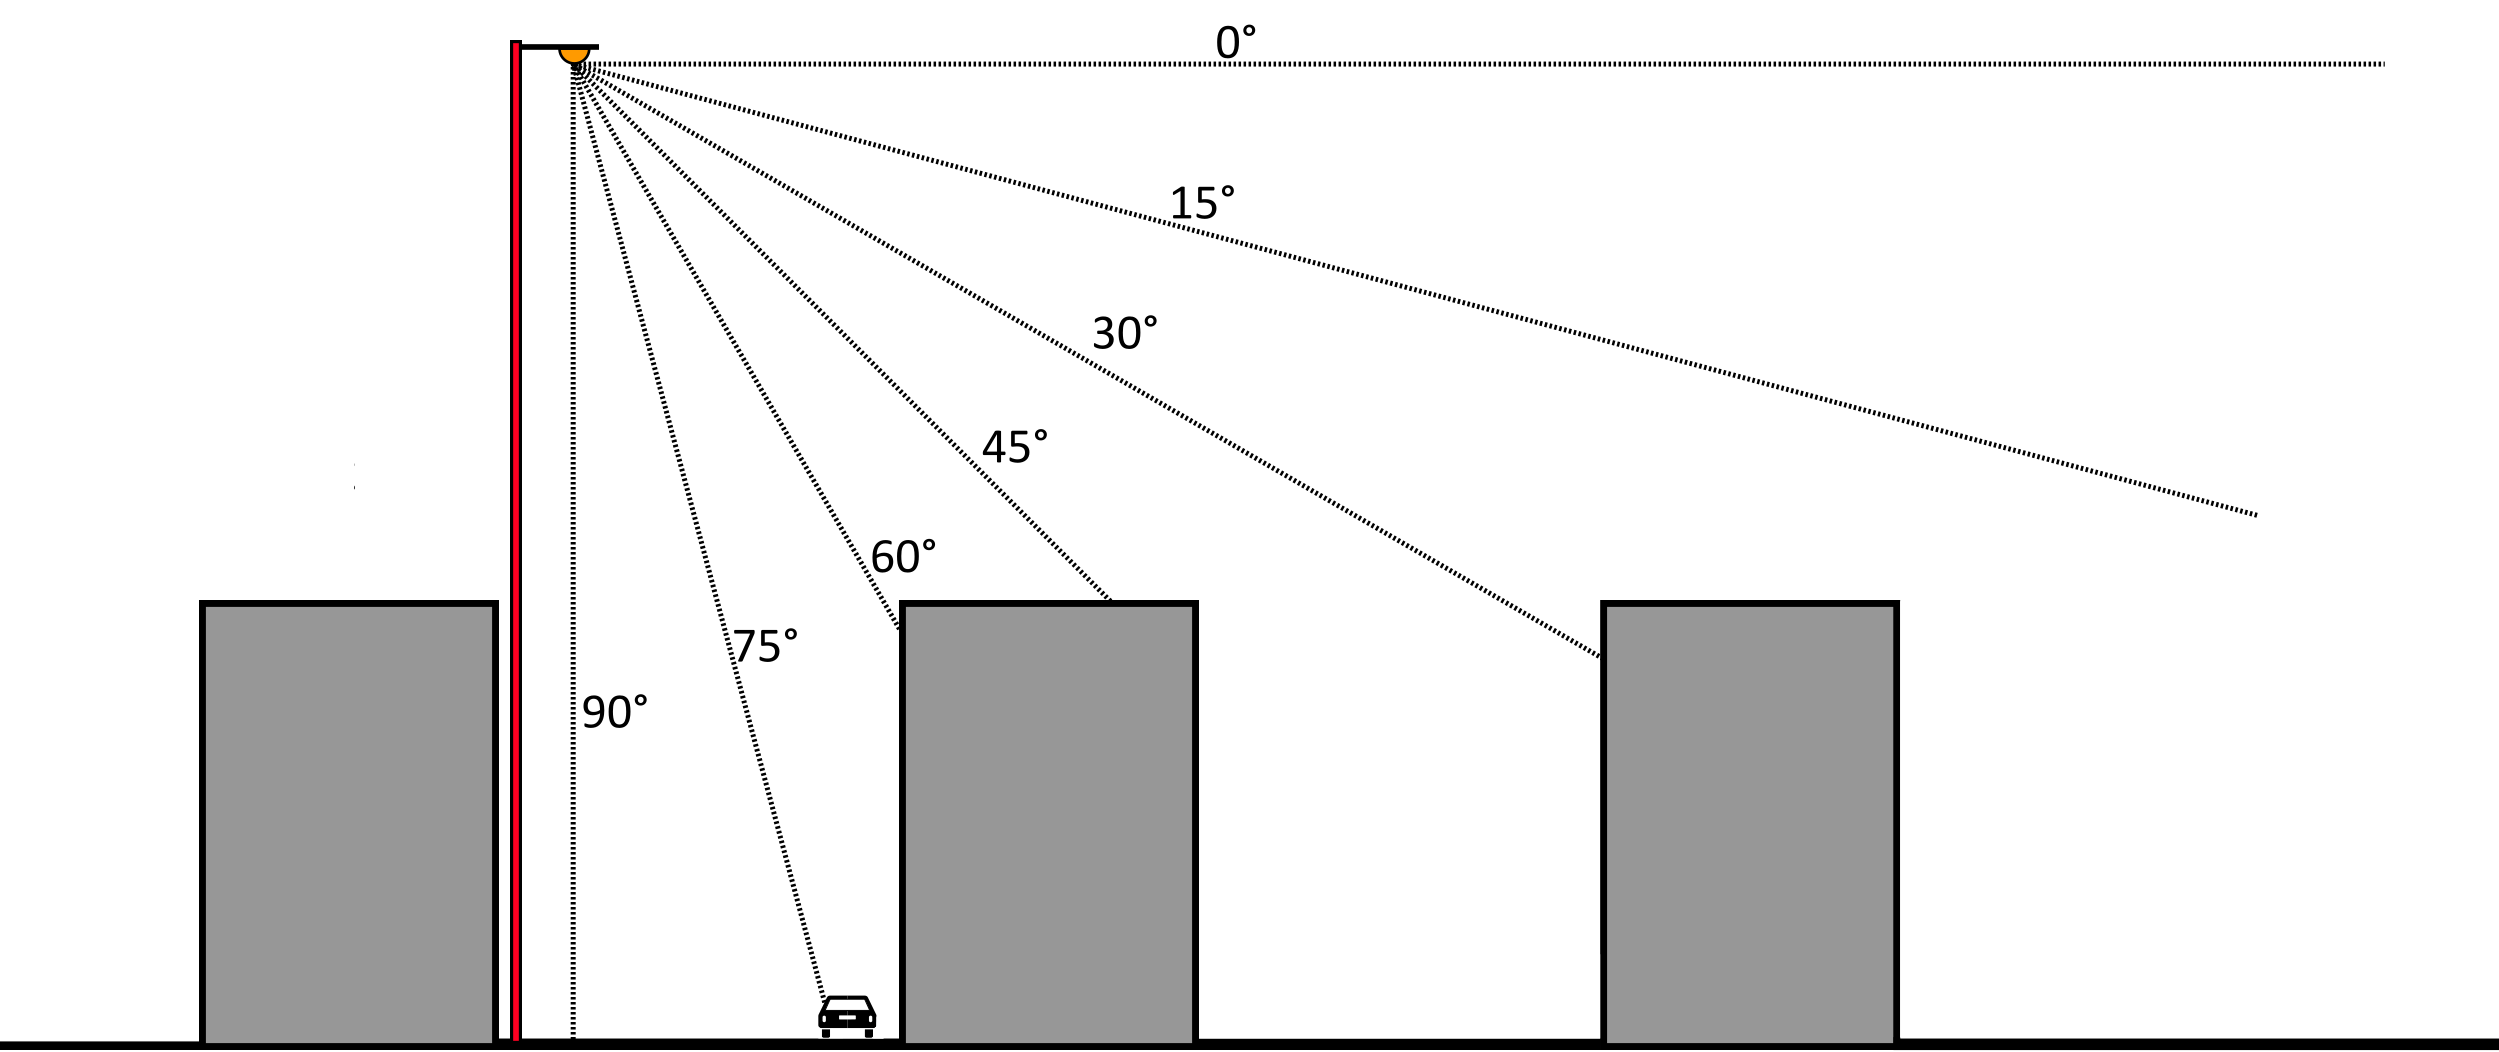
\includegraphics[width=\textwidth]{lineofsight}
	\label{lineofsight}
	\caption{Variable path geometry inherent with wide-FOV near-ground sensor visualized over an idealized 2-dimensional urban area.}
\end{figure}

Several multi-LOS atmospheric correction routines have been developed for near-ground TIR: Meier et al., 2011 describes a correction method for oblique angled urban thermography \cite{Meier2011}. Path lengths were calculated for each pixel over the FOV of a tower-mounted thermal imager angled obliquely toward the urban surface. A correction factor was then computed and applied using a radiative transfer code initialized using isothermal, isohumal atmospheric profiles for each time step. Applied over a time-series of images, the result is a continuous atmospherically corrected series of thermal images with each pixel representing a different T\textsubscript{rad}. However, the method uses visual-band images and a GIS database to represent urban geometry for each pixel's LOS - a technique not possible with a pyrgeometer, which returns a single integrated irradiance at each time-step. Moreover, the target instrument operates over a narrow waveband, reducing the magnitude and variance in atmospheric transmission over the sensor response curve. Thus, the method is not directly generalizable to correction TIR as measured via pyrgeometer.  Kotani \& Sugita, 2009 describes a method for correction of wide-FOV (pyrgeometer) TIR Irradiances \cite{Kotani2009a} over planar terrain. However, these methods are limited to narrow-FOV thermal imagers and sensors over planar surfaces respectively. A method which combines Meier et al., 2009's representation of complex surface geometry and Kotani \& Sugita, 2009's broadband hemispherical integration is needed for atmospheric correction of urban TIR measured from a downward facing pyrgeometer. A method to correct hemispherical broadband TIR as measured from a downward facing pyrgeometer needs to combine the two for accurate T\textsubscript{hem} retrieval over rough terrain. 

\section{A "rolling lookup table" method for hemispherical atmospheric correction}

%alt title:method to retrieve atmospherically corrected hemispherical surface temperatures from near ground TIR

The "rolling lookup-table" method described in this study uses a sensor view model in conjunction with a radiative transfer code to model hemispherical irradiances upwelling from a simplified isothermal 3-dimensional representation of the target study area. In summary, the method (depicted in figure \ref{flow}) uses vertical profiles of measured T\textsubscript{air} and humidity to model at-sensor spectral radiances at 5$^{\circ}$ increments over the sensor FOV for a predefined range of possible T\textsubscript{hem} at each time-step. Spectral directional radiances are convolved by a dome transmittance curve, integrated over the sensor waveband, and weighted for their respective angular view factor. Weighted directional radiances are then integrated over the hemisphere and aggregated into a lookup table (LUT) of modeled irradiance---T\textsubscript{hem} pairings for each timestep, unique to the vertical profile of measured T\textsubscript{air} and humidity. Finally, for each time-step, measured irradiances are matched with the closest modeled irradiances in the associated LUT to return an atmospherically corrected hemispherical surface temperature (T\textsubscript{hem}). This process is repeated at 30 minute intervals to yield a continuous climatology of urban T\textsubscript{hem} for surface urban heat island (sUHI) analysis. The following sections introduce the study area and describe the sensor view modeling, radiative transfer, and post-processing steps of the method.



\begin{figure}[!ht]
	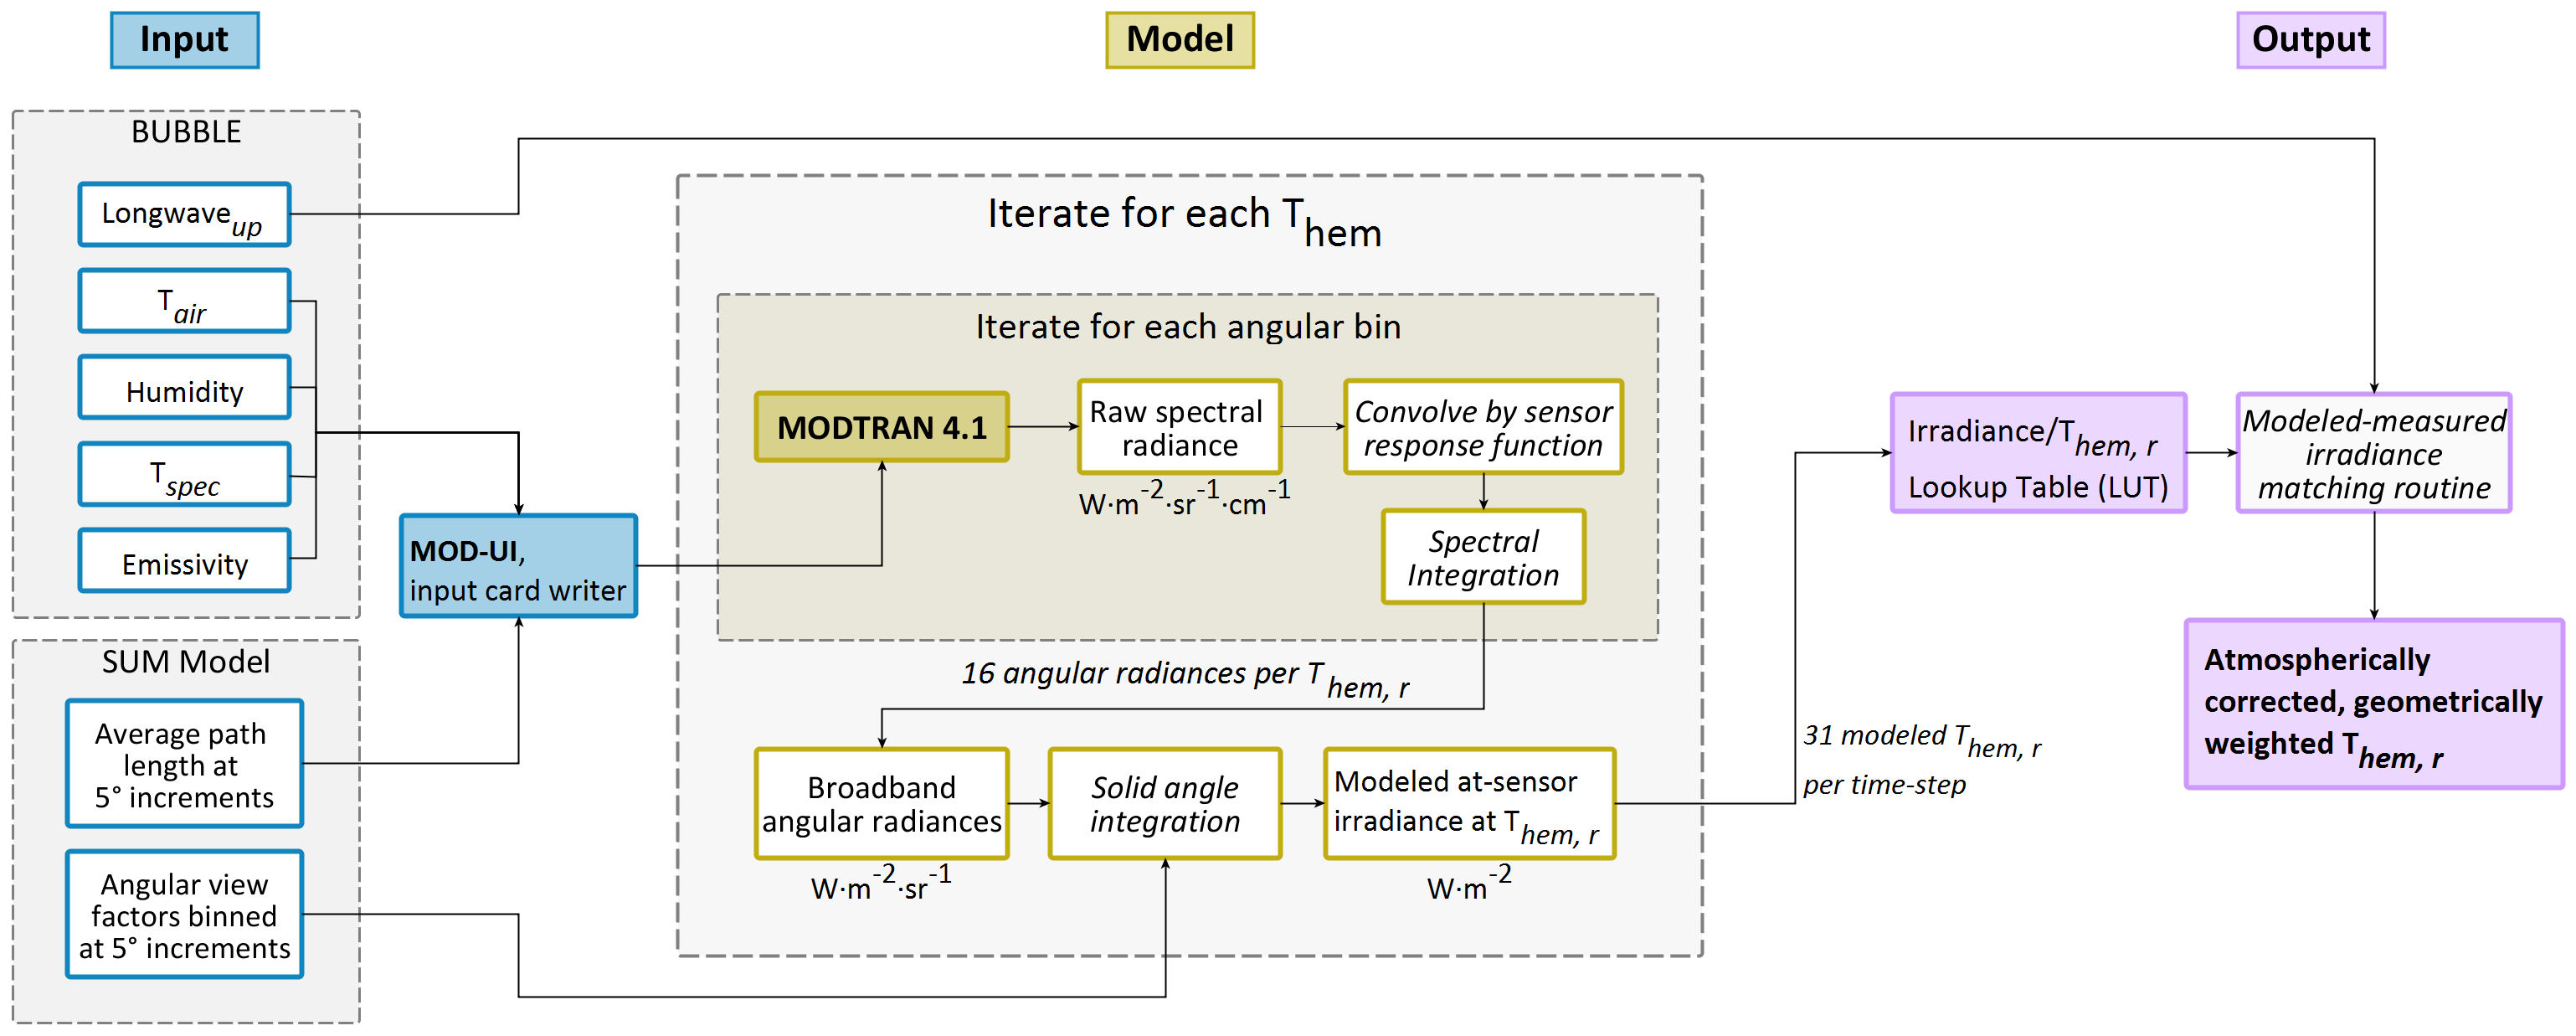
\includegraphics[width=\textwidth]{flow}
	\label{flow}
	\caption{A workflow schematic depicting the input, model, and output-processing steps of a "rolling lookup table method" for hemispherical radiometric surface temperature retrial.}
\end{figure}

\subsection{Study area}

As discussed in Section \ref{Atmospheric correction of near-ground TIR}, atmospheric correction of longwave irradiances measured from downward-facing, near-ground, wide-FOV sensors must account for surface geometry - particularly when mounted to view complex surface geometry. Hence, routines to retrieve atmospherically corrected urban T\textsubscript{hem} from upwelling longwave irradiances are inherently site specific. However, it is important to note that although correction magnitudes described in this paper are not generalizable, the correction method described in this paper can readily be adapted to different study sites, pyrgeometer types, and unique surface geometries.

With methodological generalizability in mind, a "rolling lookup table" atmospheric correction method was developed to retrieve radiometric T\textsubscript{hem} for a climatology of upwelling longwave irradiances measured from above the Sperrstrasse urban street canyon in Basel, Switzerland. The site, instrumented as a part of the Basel Urban Boundary Layer Experiment (BUBBLE) \cite{Rotach2005}, has an approximately northeast-southwest orientation and site morphology representative of local climate zone (LCZ) 2\footnote{Site surroundings can be described by the following morphological parameters: mean building height: 14.6m, plan aspect ratio: 0.54, complete aspect ratio: 1.92, local canyon aspect ratio: 1.0, and average shortwave albedo: 0.11 \cite{Rotach2005}.} \cite{Stewart2012}. LCZ classification was based on an assessment of surface characteristics in a 250m circular area extending from the Sperrstrasse tower using a 1m raster digital building model (DBM). Thus, the morphological parameters identified in \cite{Rotach2005} are representative of the vast majority of the pyrgeometer footprint. However, it should be noted that vegetation was not included in the DBM, and thus is not represented in morphological assessment or the sensor view model. 

For the nine month period between November 2001 and July 2002, a triangular lattice tower was installed skewed towards the southeast facing wall near the center of the Sperrstrasse canyon to observe a full suite of meteorological, radiation, and flux parameters. Profiles of T\textsubscript{air} and humidity were measured from seven heights extending from 2.5m to 31.5m above the canyon floor (with the highest observation level at approximately 2.17 times mean building height). Upwelling and downwelling short/longwave fluxes were measured at the lowest and highest tower heights, with an additional downward facing pyrgeometer mounted at roof level in the center of the canyon. In addition, during a summertime intense operation period (IOP) an array of narrow-FOV IRTs was installed to view individual facet surface temperatures (T\textsubscript{facet}) of approximately the same urban patch viewed by the pyrgeometer. 

The BUBBLE Sperrstrasse site was chosen for two primary reasons: 1. The study site provided a long-term climatology of radiation and meteorological variables for a representative mid-latitude city over a diverse range of synoptic conditions. This allowed for examination of urban T\textsubscript{surf}, atmospheric correction magnitudes, and sUHI magnitudes over a wide range of mid-latitude conditions. 2. T\textsubscript{facet} measured during the summertime IOP allowed for direct climatological comparison of T\textsubscript{hem} to wall (T\textsubscript{wall}), roof (T\textsubscript{roof}), and road (T\textsubscript{road}) surface temperatures of both the northwest- and southeast-facing sides of the canyon. In addition, several hypothetical sensor views of the canyon were simulated by weighting to represent different geometric representations of the canyon, including a nadir/plan view, an oblique south-facing, and an oblique north-fac from narrow-FOV sensors and a complete, 3-dimensional view of the canyon. This facilitated comparison of T\textsubscript{hem} against different instrument types and platforms to identify and quantify biases in each method.  In each representation, different weightings were applied to T\textsubscript{wall}, T\textsubscript{roof}, and T\textsubscript{road} on both sides of the canyon to represent different sensor orientations and sampling regimes. Weightings for each representation are described in table \ref{weightings}. 
\begin{table}[!ht]
	\centering
	\caption{Weightings to produce T'\textsubscript{rad} for different geometric representations of the Basel street canyon.}
	\label{weightings}
	\begin{tabular*}{\textwidth}{l@{\extracolsep{\fill}} p{1cm}p{1cm}p{1cm}p{1cm}p{1.6cm}}
		\toprule 
		& Road & Northwest & Southeast & Northwest & Southeast \\ 
		&  & Roof & Roof & Wall & Wall \\ 	\midrule

		Complete & 0.33 & 0.16 & 0.16 & 0.16 & 0.16 \\ 

		Nadir & 0.46 & 0.27 & 0.27 & 0.00 & 0.00 \\ 

		Oblique (south-facing) & 0.20 & 0.25 & 0.25 & 0.00 & 0.30 \\ 

		Oblique (north-facing) & 0.20 & 0.25 & 0.25 & 0.30 & 0.00 \\ 
		\bottomrule
	\end{tabular*} 
\end{table}

\subsection{Modeling path lengths of 3-dimensional terrain}

The sheer number of unique path length geometries inherent with wide-FOV radiometry of rough terrain makes full 3-dimensional radiative transfer simulation difficult and computationally intensive --- particularly when correcting a climatology of T\textsubscript{hem}. In this method, to improve model efficiency, radiances are calculated for azimuthally averaged path lengths that represent average surface terrain for each solid angle "slice" of the sensor FOV. Thus, hemispherical radiative transfer is reduced to a 2-dimensional problem (shown in panel (b) of figure \ref{23radtran}). This greatly reduces the computational time required to model each irradiance-T\textsubscript{hem} pairing, as angular radiances can be computed as a function of zenith angle alone and subsequently weighted and integrated 3-dimensionally over the hemisphere. 

To calculate surface-sensor geometries, the Surface-Sensor-Sun Urban Model (SUM) \cite{Soux2004} is initialized with a simplified, orthogonal 3-dimensional DBM representing the street canyons and courtyards immediately surrounding the sensor. SUM uses a four-dimensional array to represent surface morphology   with three spatial dimensions ($x$, $y$, and $z$), with $z$ representing height above the $x$, $y$ plane. SUM also includes an additional fourth dimension, where properties describing each cell are stored (in this case, distance from the point to the sensor). After specifying sensor FOV and position relative to the DBM, the model determines which patches have an unobstructed line of sight to the sensor and calculates the distance from "seen" patches to the sensor. Path lengths are binned at 5$^{\circ}$ increments of zenith angle and averaged to return an azimuthally-independent mean path length for each bin. In addition, while simulating path length geometries, SUM calculates view factors for each solid angle "slice", which are later used to weight 2-dimensional angular radiances in the hemispherical integration post-processing steps.

\begin{figure}[!ht]
	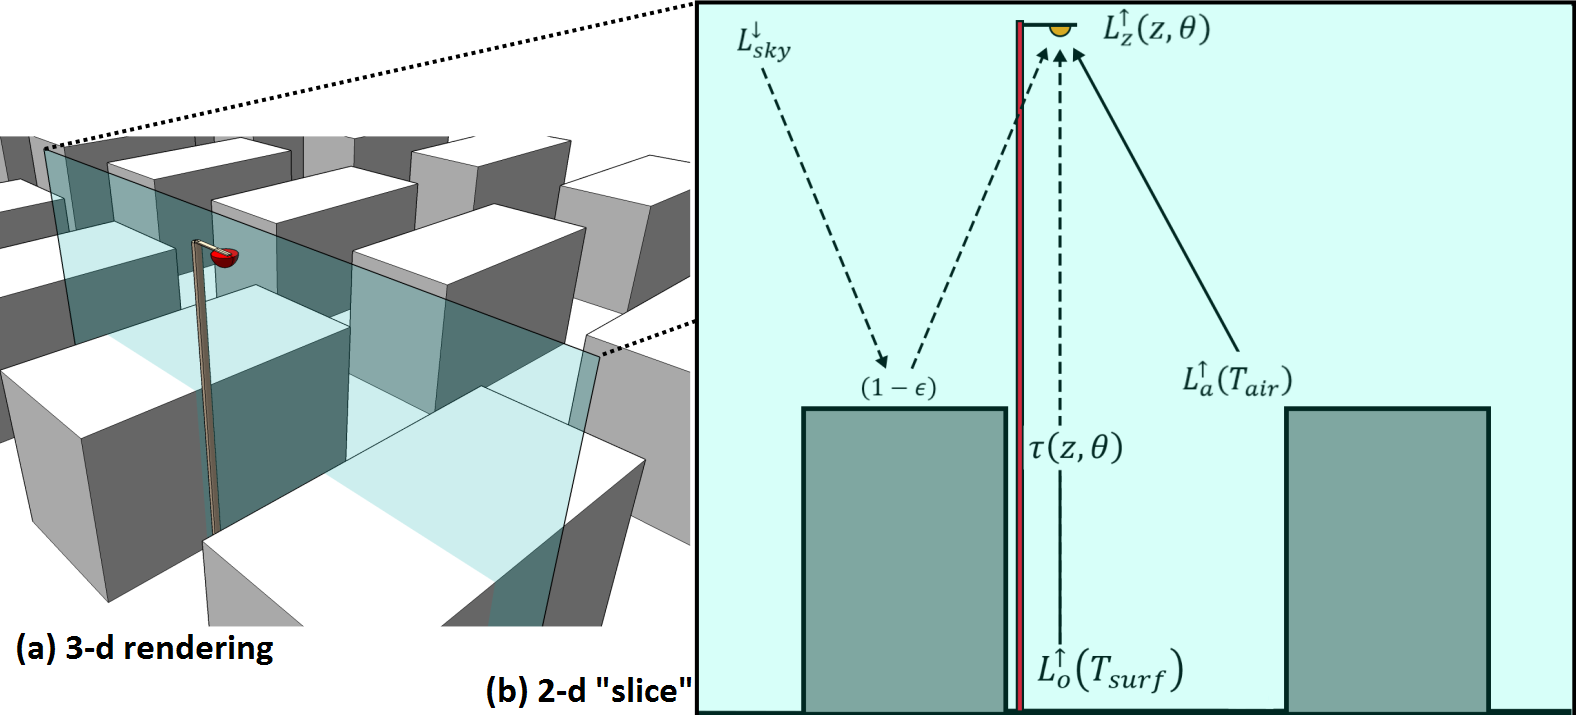
\includegraphics[width=\textwidth]{23radtran}
	\label{23radtran}
	\caption{A typical 2-dimensional (b) radiative transfer schematic adapted for an idealized 3-dimensional urban area (a). In 3-dimensions, path length for a given zenith angle can change significantly with azimuth angle. Dotted lines indicate the potential for absorption by the intervening atmospheric layer}
\end{figure}

\subsection{Modeling hemispherical irradiances}
With path length geometries calculated in SUM, irradiances are modeled time-sequentially using the MODerate resolution atmospheric TRANsmission 4.1 radiative transfer code (MODTRAN) \cite{Berk1987}. At each time-step, a range of potential T\textsubscript{hem} is selected using T\textsubscript{bright} subtracted by some constant (6 K during nighttime runs and 4 K for daytime runs). In MODTRAN, at-sensor spectral radiances for each path length are modeled over a waveband of 0---2500cm\textsuperscript{-1} at 0.5 K intervals over the range of potential T\textsubscript{hem}. Atmospheric profiles are constructed from 30-minute averages of T\textsubscript{air} and humidity with aerosol and above-sensor conditions are informed by the mid-latitude summer standard atmosphere when daytime maximum T\textsubscript{air} is greater than 10 $^{\circ}$C (the mid-latitude winter profile is substituted on days with T\textsubscript{air, max} of less than 10 $^{\circ}$C). 
Spectral radiances are convolved by a dome transmittance.




\section{Evaluation of the method using profiles of upwelling longwave radiation over a homogenous planar surface}

MODTRAN has been shown to effectively model near-ground radiative transfer at urban-scale path lengths in 2-dimensions. However, the method detailed in this paper includes significant post-processing to ‘collate’ point-to-point radiances into 3-dimensional hemispherical irradiances. In addition, the method accounts for site-specific surface geometry, which has a significant influence on boundary-layer transmittance of broadband longwave radiation. Thus, prior to deriving a climatology of radiometric urban Them, the method was evaluated over a simple surface with known surface characteristics. Thus, divergences are solely the result of differential atmospheric effects with increasing height above ground, which should be accounted for by the model. It is assumed that each pyrgeometer in this validation views a patch with approximately the same temperature. 

Profiles of upwelling longwave radiation, downwelling shortwave, air temperature, and humidity at 2m, 10m, and 30m were obtained from the Payerne station, located 50 miles southwest of Basel, Switzerland in a cultivated field. To evaluate the method, we used a modified version of the workflow described in XXXX. Brightness temperature calculated from the lowest upwelling longwave measurement was used to model irradiances at 10m and 30m at each time-step. Downwelling shortwave radiation was used to categorize test days based on cloud cover. The daytime air temperature profile was modified to replicate typical lapse rates in the Sperrstrasse canyon. Unlike, Kotani \& Sugita (2009), an isothermal atmospheric profile was not sufficient to accurately model upwelling longwave divergences (nor fluxes) of planar terrain. Although thermal stratification is likely to be relatively small by day in an urban canyon \cite{Nakamura1988} --- where strong microscale contrasts in Tsurf foster canyon mixing and neutral stability --- the large daytime Tsurf-T\textsubscript{air}  differential and the path-length/transmittance gradient can create large positive divergences (5 – 15 Wm\textsuperscript{-2},CHECK THIS). As such, we suggest using a full canyon T\textsubscript{air} /humidity profile to 

Modeled upwelling longwave at 10m and 30m and divergences are compared to their measured counterparts in figure a. Both fluxes and divergence show strong correlations, thus we conclude: 1. Irradiances measured at 2m are free from significant atmospheric influence – as an uncorrected irradiance provided an accurate Tsurf for modeling of 10m and 30m Irradiances As such, brightness Them and radiometric Them are approximately equal when z < 2m. Although, it should be noted that a 2m sensor is not representative of canyon geometry and should not be used to derive urban Them. 2. The method is sensitive enough to model divergences in a large layer above a flat surface. Urban divergences are likely to be smaller with less frequent and less severe stable stratifications. Thus, we can safely make the assumption that the method is effective over complex terrain – provided path length geometries are accurately replicated in SUM.


